\chapter{Resultados}
\label{chap:resultados}

\drop{E}{n} el siguiente capítulo se presentan los resultados obtenidos tras desarrollar el
sistema. Para ello se hace un análisis de los recursos que consume y el coste económico
de desarrollarlo. Además se especifica paso a paso un caso de uso en concreto. Finalmente se
proporciona la dirección del repositorio donde están contenidos todos los archivos del proyecto.

\section{Recursos y costes}

En esta sección se desglosarán los recursos y los costes empleados en el sistema. Por un lado
presentaremos las estadísticas del proyecto, por otro una estimación del coste de acuerdo a las
condiciones actuales del mercado y, finalmente, algunas medidas de rendimiento del sistema.

\subsection{Estadísticas}

En la tabla~\ref{cuadro:lineasCodigo} se muestra el número de lineas de código del proyecto
\emph{Naviganto} completo. Para contabilizar dichas líneas se ha empleado el comando \texttt{cloc}.

\begin{table}[h]
  \centering
  \begin{tabular}{|l|r|r|r|r|}
    \hline
    \textbf{Lenguaje} & \textbf{Archivos} & \textbf{Espacios en blanco} & \textbf{Comentarios} & 
      \textbf{Líneas de código} \\
    \hline
    \emph{XML}                &         662  &         2231  &          4524  &         26220  \\
    \hline
    \emph{Java}               &          28  &         1312  &          9265  &          7023  \\
    \hline
    \emph{Bourne Again Shell} &           1  &           20  &            21  &           123  \\
    \hline
    \emph{DOS Batch}          &           1  &           24  &             2  &            64  \\
    \hline
    \emph{IDL}                &           1  &            2  &             0  &            15  \\
    \hline
    \textbf{Total}            & \textbf{693} & \textbf{3589} & \textbf{13812} & \textbf{33445} \\
    \hline
  \end{tabular}
  \caption{Número de líneas de código fuente de Naviganto por lenguajes}
  \label{cuadro:lineasCodigo}
\end{table} 

\subsection{Coste económico}

El desarrollo del proyecto \emph{Naviganto} empezó aproximadamente el día 3 de Noviembre de 2014 y
terminó alrededor del 9 de Enero de 2015, es decir, unas 10 semanas de desarrollo. Con una
dedicación media de 6 horas diarias y 5 días a la semana, da como resultado un total de 300 horas de
trabajo. Todo ello sin contabilizar el tiempo dedicado a la elaboración del presente documento.

Tomando como referencia la media en España de unos 16 \euro/hora para los analistas y
desarrolladores sin experiencia
laboral~\footnote{http://www.tusalario.es/main/salario/comparatusalario} y los elementos
\emph{hardware} necesarios (ver sección~\ref{sec:herramientasHardware}) para el desarrollo, se ha
elaborado el cuadro~\ref{cuadro:costes} con una estimación del coste.

\begin{table}[h]
  \centering
  \begin{tabular}{|l|r|r|}
    \hline
    \textbf{Recurso} & \textbf{Cantidad} & \textbf{Coste} \\
    \hline
    Sueldo del programador (300 horas)     & 1 &          4800 \euro \\
    \hline
    Computador de trabajo                  & 1 &           499 \euro \\
    \hline
    Smartphone de la aplicación principal  & 1 &           399 \euro \\
    \hline
    Smartphone de la aplicación bluetooth  & 2 &            60 \euro \\
    \hline
    Smartwatch de la aplicación wear       & 2 &           239 \euro \\
    \hline
    \textbf{Total}                         &   & \textbf{6296} \euro \\
    \hline
  \end{tabular}
  \caption{Desglose de costes del desarrollo de Naviganto}
  \label{cuadro:costes}
\end{table}

El coste obtenido es puramente informativo ya que para calcular el presupuesto real se deben tener
en cuenta otros muchos factores. De todos modos, es de suponer que el coste del desarrollo de
\emph{Naviganto} se ajustará más al cuadro~\ref{cuadro:costes} que a la estimación ofrecida del
comando \texttt{sloccount} (ver listado~\ref{code:cocomo}) que calcula el tamaño del proyecto en
líneas de código y emplea el modelo \acf{COCOMO} para obtener la estimación del tiempo y los costes
necesarios para desarrollar el sistema.

\begin{listing}[
  float=ht,
  caption  = {Estimación de los costes del desarrollo de Naviganto según sloccount},
  label    = code:cocomo]
Total Physical Source Lines of Code (SLOC)                = 32,085
Development Effort Estimate, Person-Years (Person-Months) = 7.63 (91.59)
 (Basic COCOMO model, Person-Months = 2.4 * (KSLOC**1.05))
Schedule Estimate, Years (Months)                         = 1.16 (13.91)
 (Basic COCOMO model, Months = 2.5 * (person-months**0.38))
Estimated Average Number of Developers (Effort/Schedule)  = 6.58
Total Estimated Cost to Develop                           = $ 1,031,000
 (average salary = $56,286/year, overhead = 2.40).
\end{listing}

\subsection{Profiling}

El \emph{profiling} o medida de rendimiento consiste en medir los tiempos que el sistema tarda en
realizar las operaciones más críticas. En el caso de \emph{Navignato} se han seleccionado las
siguientes operaciones:

\begin{itemize}
  \item Mostrar posición actual en el mapa
  \item Buscar destino cercano (\textasciitilde{}10 km)
  \item Iniciar navegación hacia un destino cercano (\textasciitilde{}10 km)
\end{itemize}

Puesto que las tres operaciones dependen tanto de la aplicación como de la conexión a Internet, se
ha desglosado en el cuadro~\ref{cuadro:conexion} la media de tiempo trascurrido tras efectuar cada
operación 10 veces sobre los diferentes tipos de conexión.

\begin{table}[h]
  \centering
  \begin{tabular}{|l|r|r|r|}
    \hline
    \textbf{Acción} & \textbf{Wifi} & \textbf{3G} & \textbf{2G} \\
    \hline
    \emph{Mostrar posición}   &  4,98 s & 6,315 s &   5,98 s \\
    \hline
    \emph{Buscar destino}     & 0,231 s & 0,407 s &  1,171 s \\
    \hline
    \emph{Iniciar navegación} & 1,086 s & 2,329 s & 25,177 s \\
    \hline
  \end{tabular}
  \caption{Desglose de tiempos de ejecución de Naviganto}
  \label{cuadro:conexion}
\end{table}

Como podemos observar, para el caso \emph{mostrar posición} existe muy poca diferencia entre las
conexiones a Internet porque el tiempo de espera viene determinado por la conexión con el satélite
\acs{GPS}. Esto es debido a que \emph{Naviganto} almacena en caché las imágenes del mapa de la
última posición en la que nos encontramos y sólo hay que esperar la posición actual.

En cambio, para \emph{buscar destino} e \emph{iniciar navegación} existe una notable diferencia de
tiempos de ejecución en función de los datos requeridos de Internet.

\section{Caso de uso concreto}
En este apartado se introducirá un caso de uso concreto del sistema funcionando por medio de
imágenes. Además, se detallará cada imagen para dar a conocer el estado en qué se encuentra el
sistema en ese momento.

En este caso de uso, nos encontramos en Campo de Criptana en la calle Virgen de Criptana nº 58 y
deseamos ir caminando hasta la Plaza Mayor. Para ello, utilizaremos nuestro \emph{smartphone} y dos
complementos vibratorios: Un \emph{smartwatch} conectado por \emph{Play Services} y un
\emph{smartphone} conectado por \emph{bluetooth}.

\subsection{Prerequisitos}

La figura~\ref{fig:hardware} muestra los componentes hardware empleados por el sistema para este
ejemplo de caso de uso. Previo inicio del sistema, las aplicaciones se encuentran instaladas en los
dispositivos del siguiente modo:

\begin{itemize}
  \item En el Nexus 5 se encuentra la aplicación principal llamada \emph{Naviganto}.
  \item En el LG G Watch R se encuentra la aplicación para \emph{wearables} llamada
    \emph{NavigantoWear}.
  \item En el Nexus One se encuentra la aplicación para hacer vibrar vía \emph{bluetooth} otros
    dispositivos Android. Se llama \emph{NavigantoBluetooth}.
\end{itemize}

Además, el usuario decide colocarse en la mano izquierda el \emph{LG G Watch R} y en el bolsillo
derecho del pantalón el \emph{Nexus One}.

\begin{figure}[!h]
  \begin{center}
    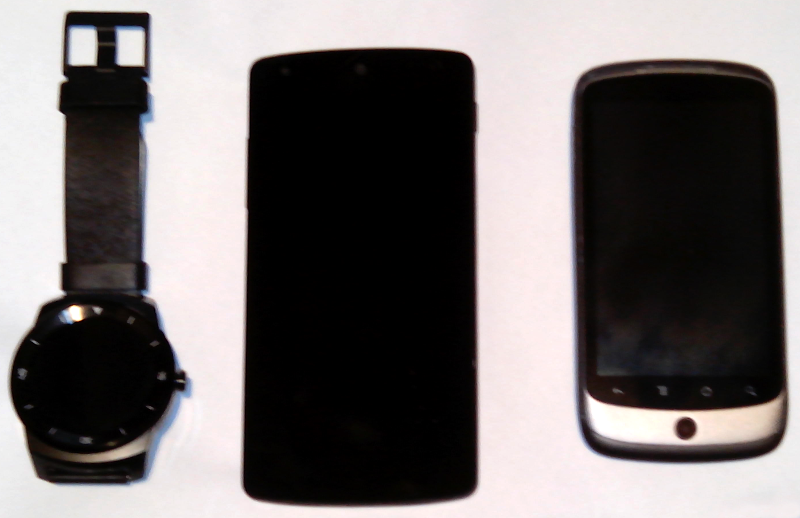
\includegraphics[width=0.7\textwidth]{/hardware.png}
    \caption{Hardware utilizado para el caso de uso concreto}
    \label{fig:hardware}
  \end{center}
\end{figure}

\subsection{Inicialización}

En la figura~\ref{fig:navigantoIni} se muestra el aspecto de \emph{Naviganto} tras iniciarse y en la
figura~\ref{fig:navigantoBarra} las diferentes opciones desarrolladas en el menú lateral.

\begin{figure}[!h]
  \begin{minipage}[b]{0.5\linewidth}
    \begin{center}
      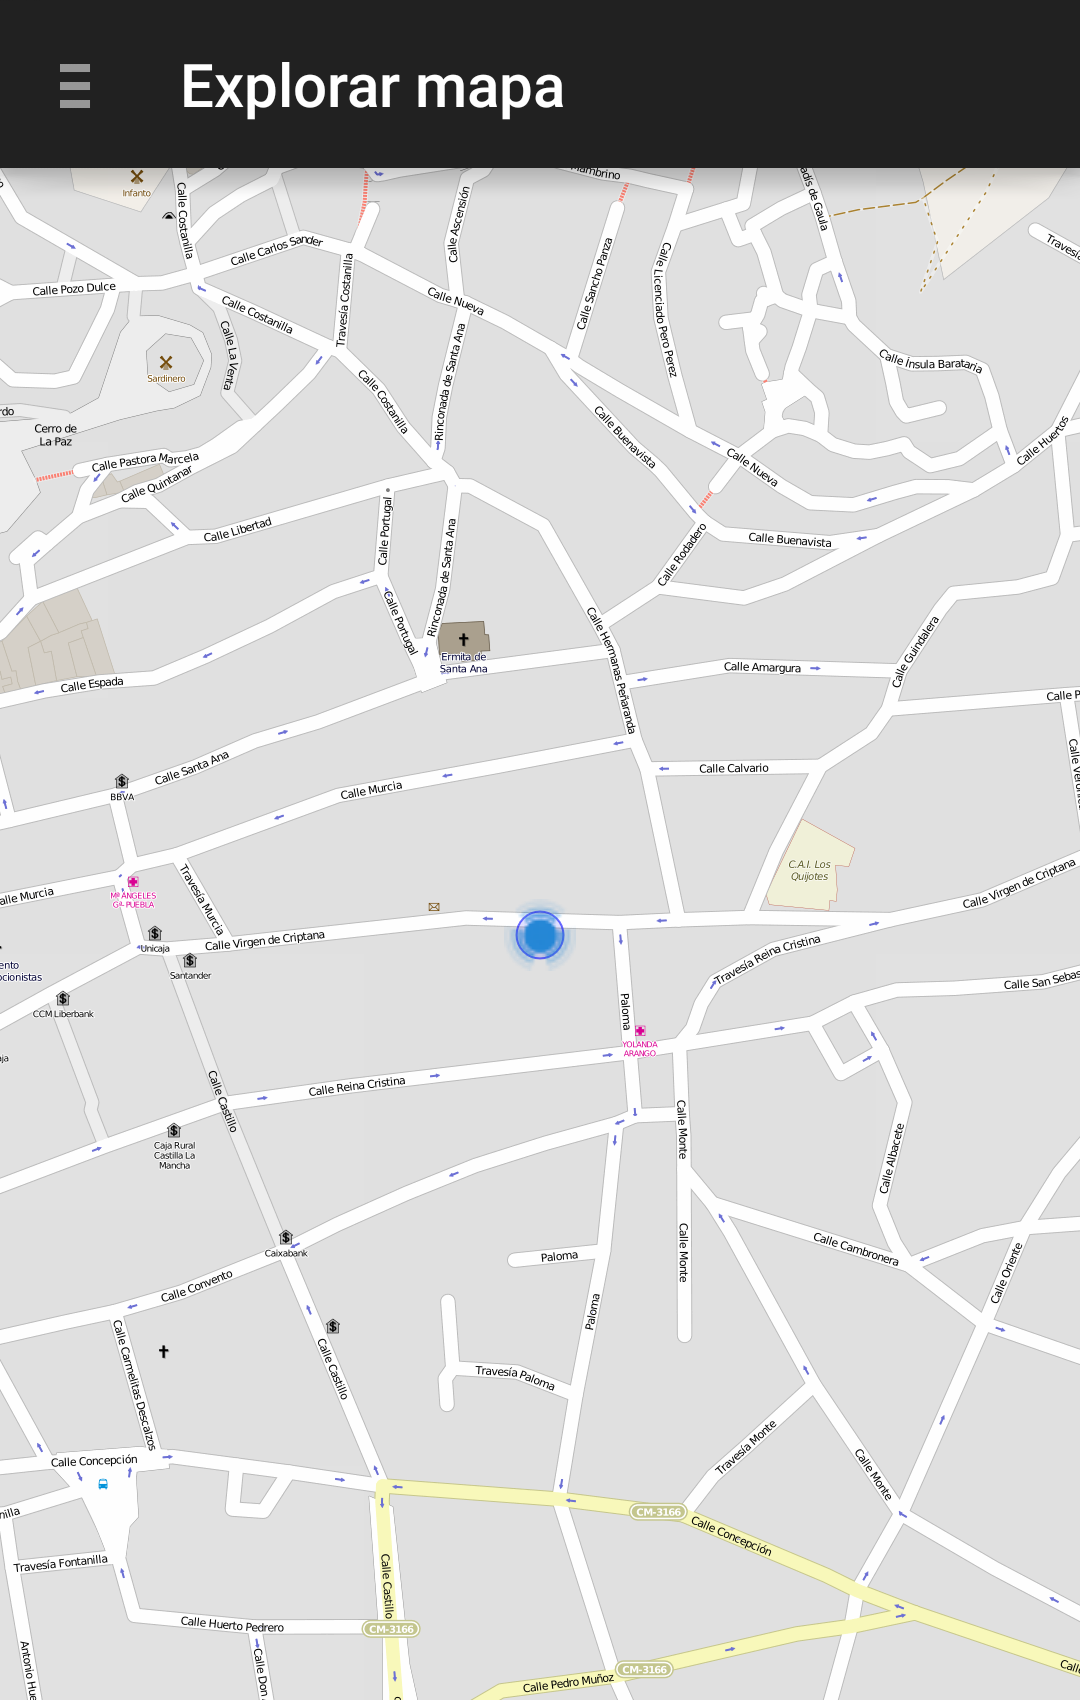
\includegraphics[width=0.85\textwidth]{/naviganto-ini.png}
      \caption{Naviganto tras iniciarse}
      \label{fig:navigantoIni}
    \end{center}
  \end{minipage}
  \begin{minipage}[b]{0.5\linewidth}
    \begin{center}
      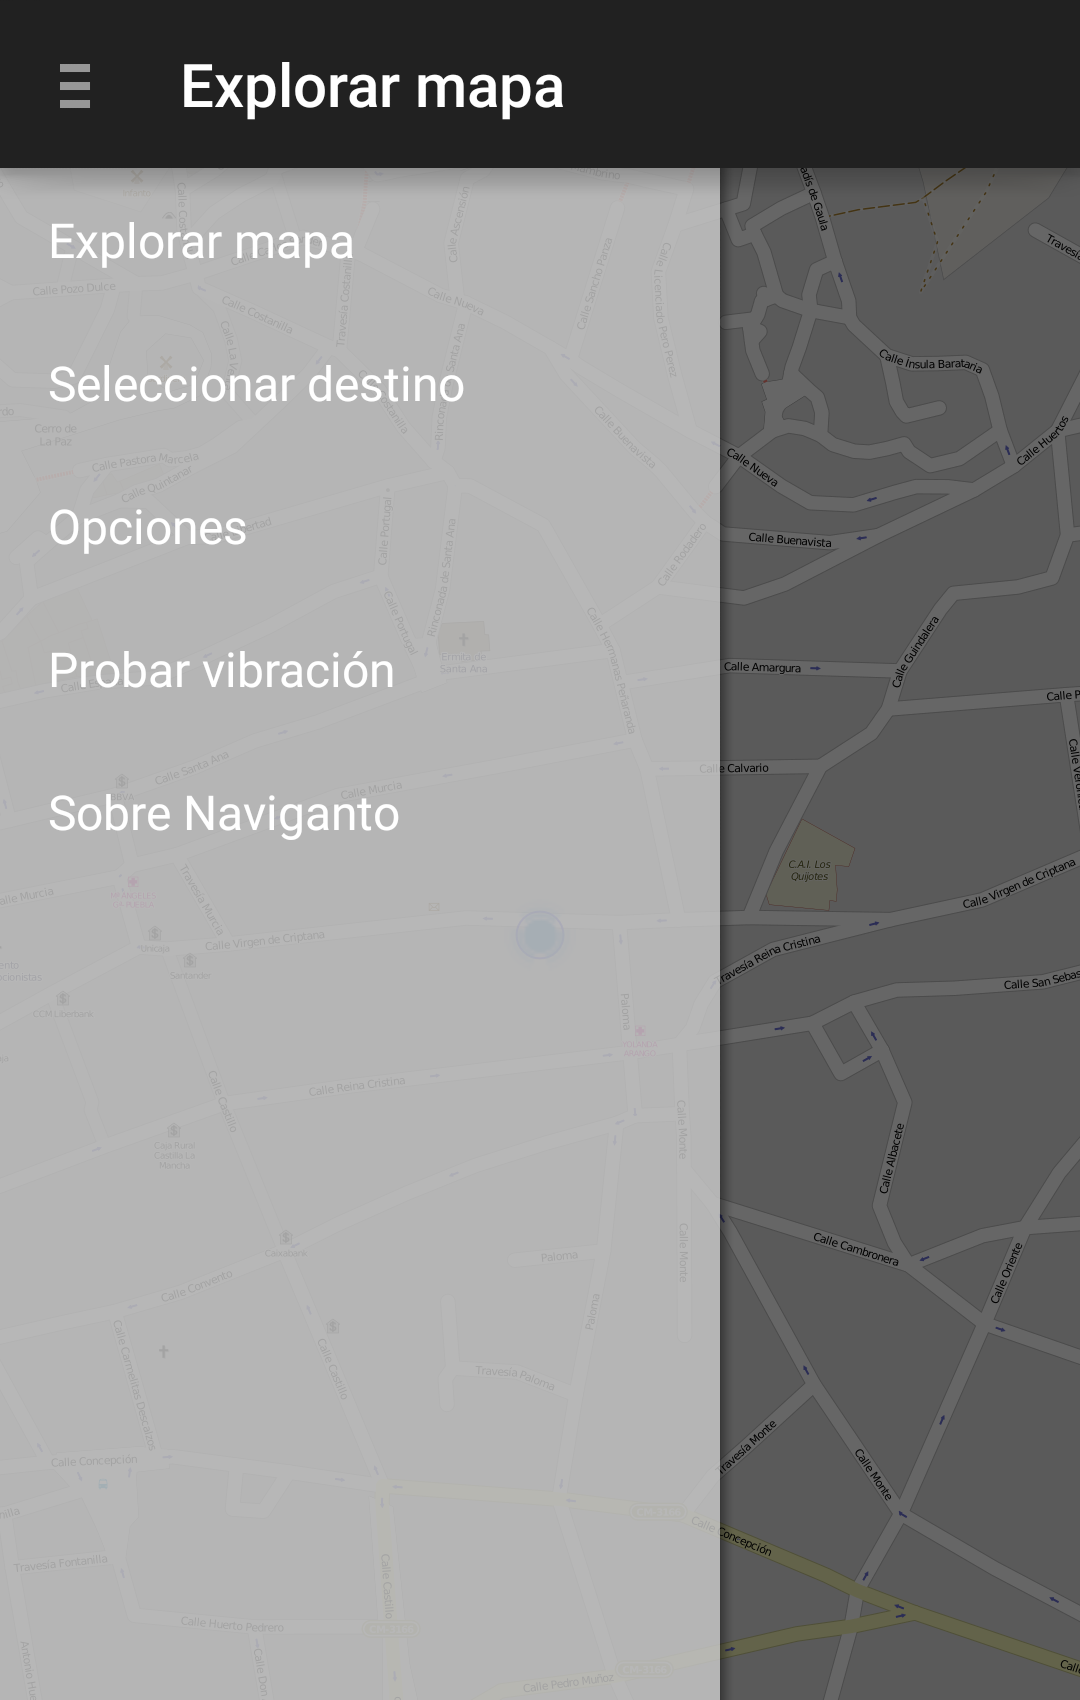
\includegraphics[width=0.85\textwidth]{/naviganto-barralateral.png}
      \caption{Barra lateral de Naviganto}
      \label{fig:navigantoBarra}
    \end{center}
  \end{minipage}
\end{figure}

\subsection{Configuración de la vibración}

Para configurar como deseamos la vibración seleccionamos en el menú lateral el apartado de
\emph{Opciones} y se nos muestra la figura~\ref{fig:navigantoOpciones} para configurar, entre otras
alternativas, la vibración. Tras activar los \emph{avisos vibratorios} (ver
figura~\ref{fig:navignatoOpcionesVibrateOn}), podemos seleccionar el \emph{Vibrador izquierdo} y el
\emph{Vibrador derecho}. Al tocar sobre cualquiera de ellos nos muestra un listado de los posibles
dispositivos (ver figura~\ref{fig:navigantoOpcionesSelecionaDispositivos}) y podemos proceder a
dejar la configuración deseada (ver figura~\ref{fig:navigantoOpcionesCasoDeUso}).

\begin{figure}[!h]
  \begin{minipage}[b]{0.5\linewidth}
    \begin{center}
      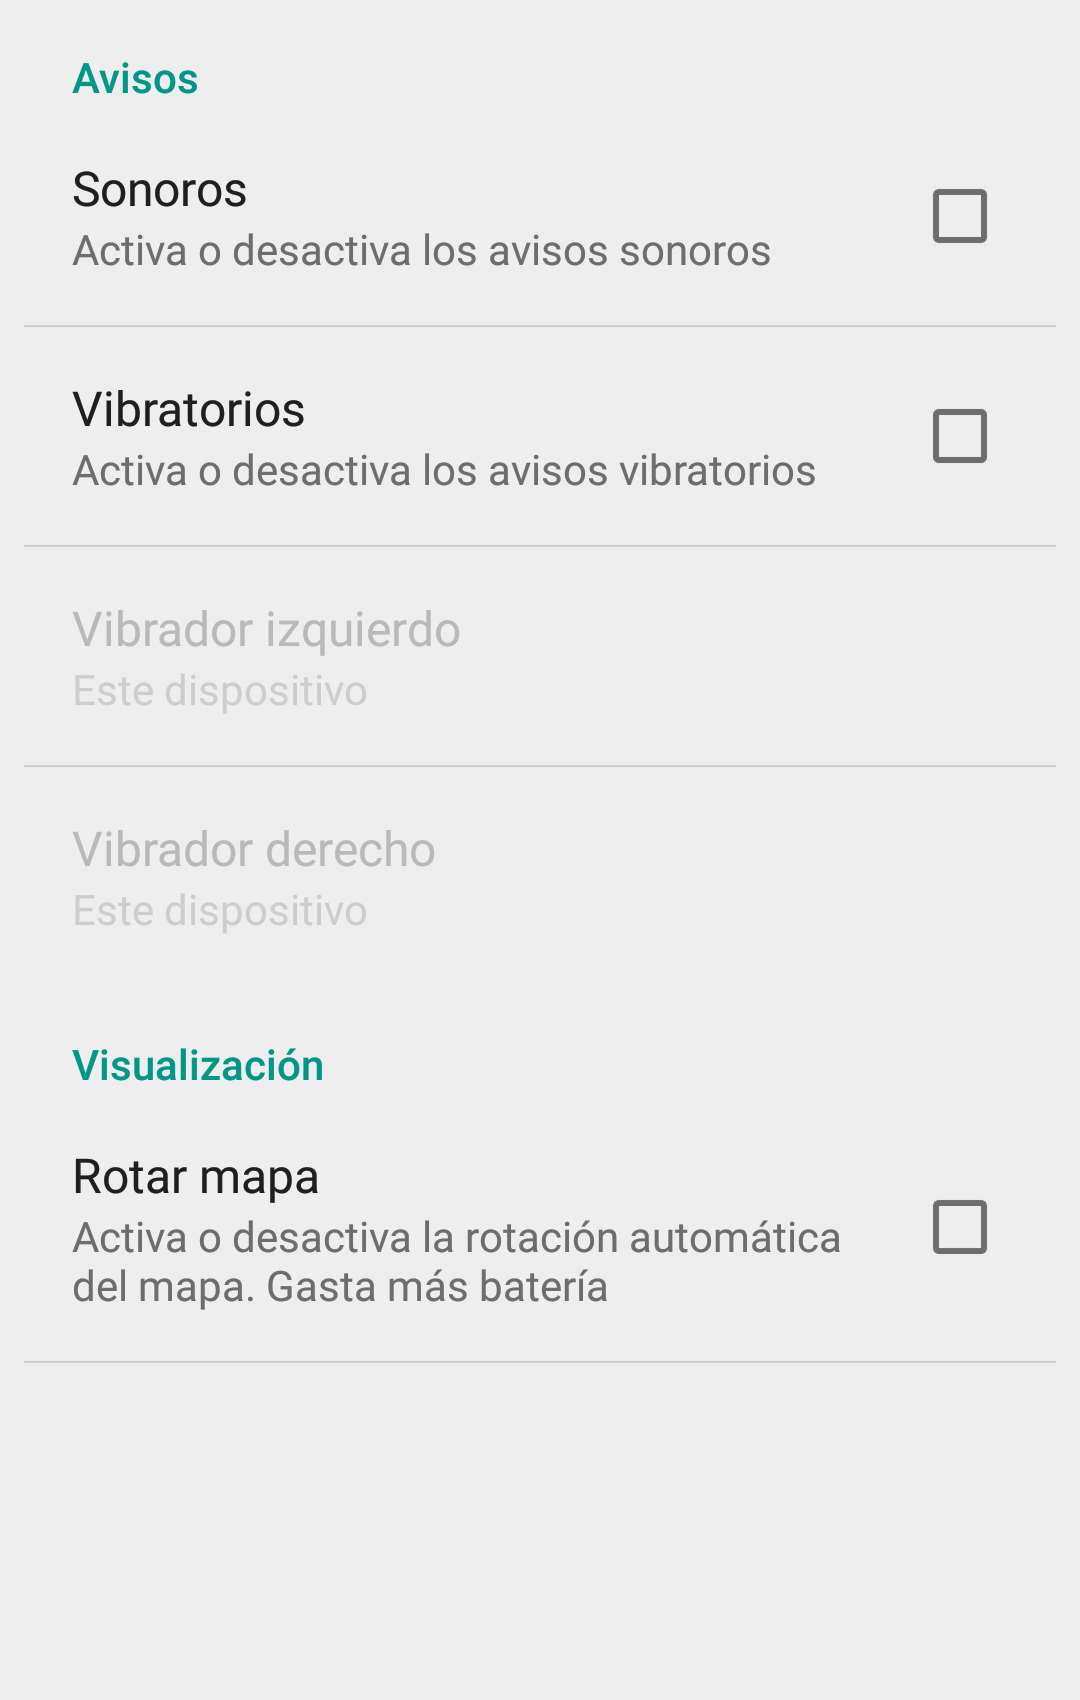
\includegraphics[width=0.85\textwidth]{/naviganto-opciones.png}
      \caption{Opciones de Naviganto}
      \label{fig:navigantoOpciones}
    \end{center}
  \end{minipage}
  \begin{minipage}[b]{0.5\linewidth}
    \begin{center}
      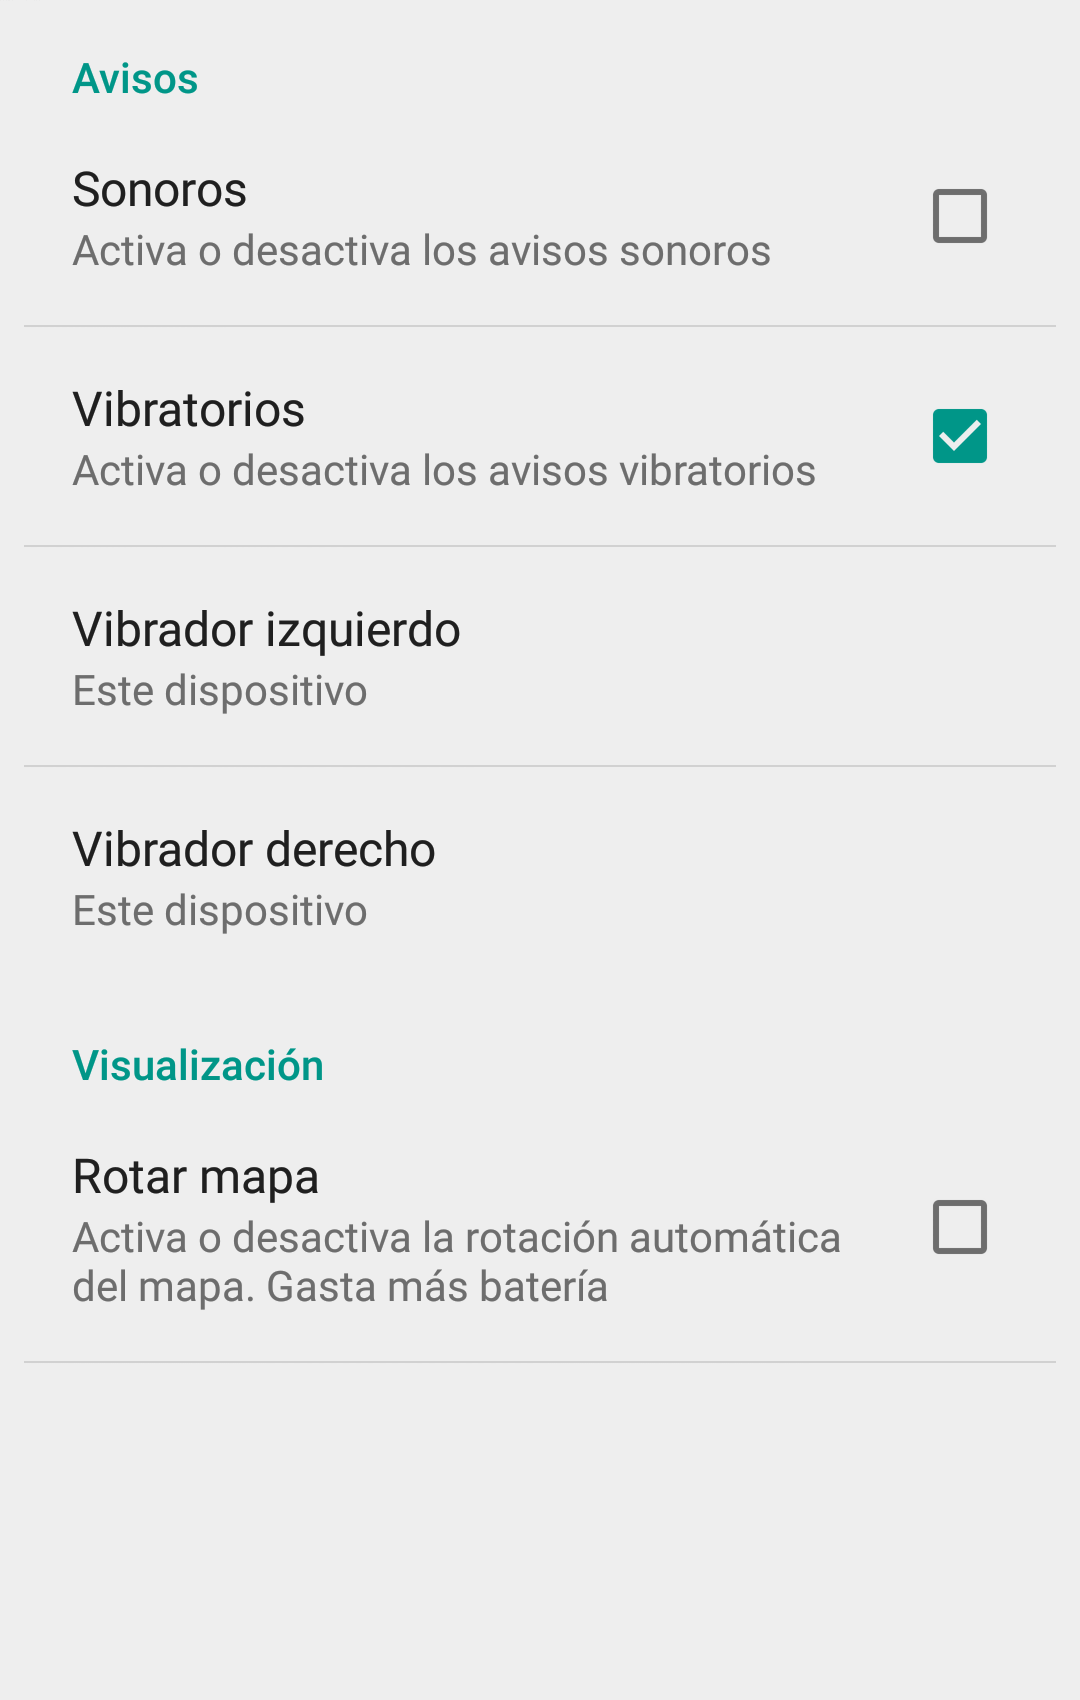
\includegraphics[width=0.85\textwidth]{/naviganto-opcionesvibrateon.png}
      \caption{Vibración activada}
      \label{fig:navignatoOpcionesVibrateOn}
    \end{center}
  \end{minipage}
\end{figure}

\begin{figure}[!h]
  \begin{minipage}[b]{0.5\linewidth}
    \begin{center}
      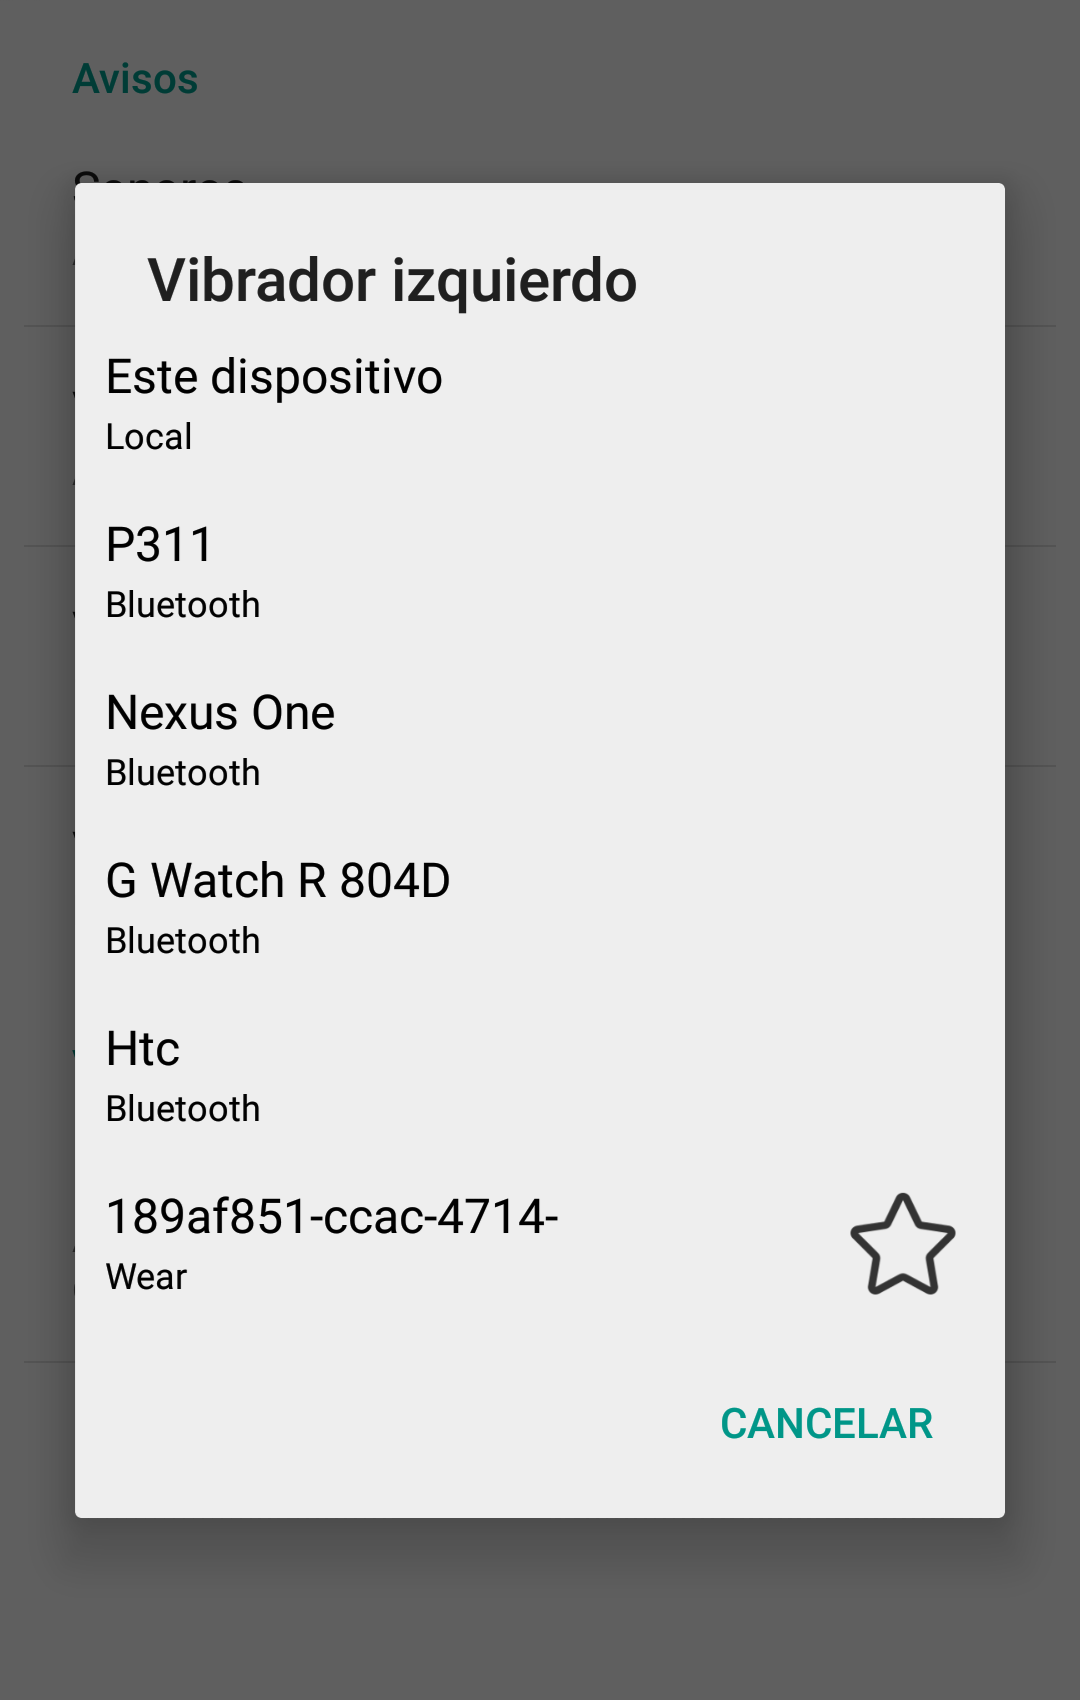
\includegraphics[width=0.85\textwidth]{/naviganto-opcioneslistadispositivos.png}
      \caption{Selección de dispositivos}
      \label{fig:navigantoOpcionesSelecionaDispositivos}
    \end{center}
  \end{minipage}
  \begin{minipage}[b]{0.5\linewidth}
    \begin{center}
      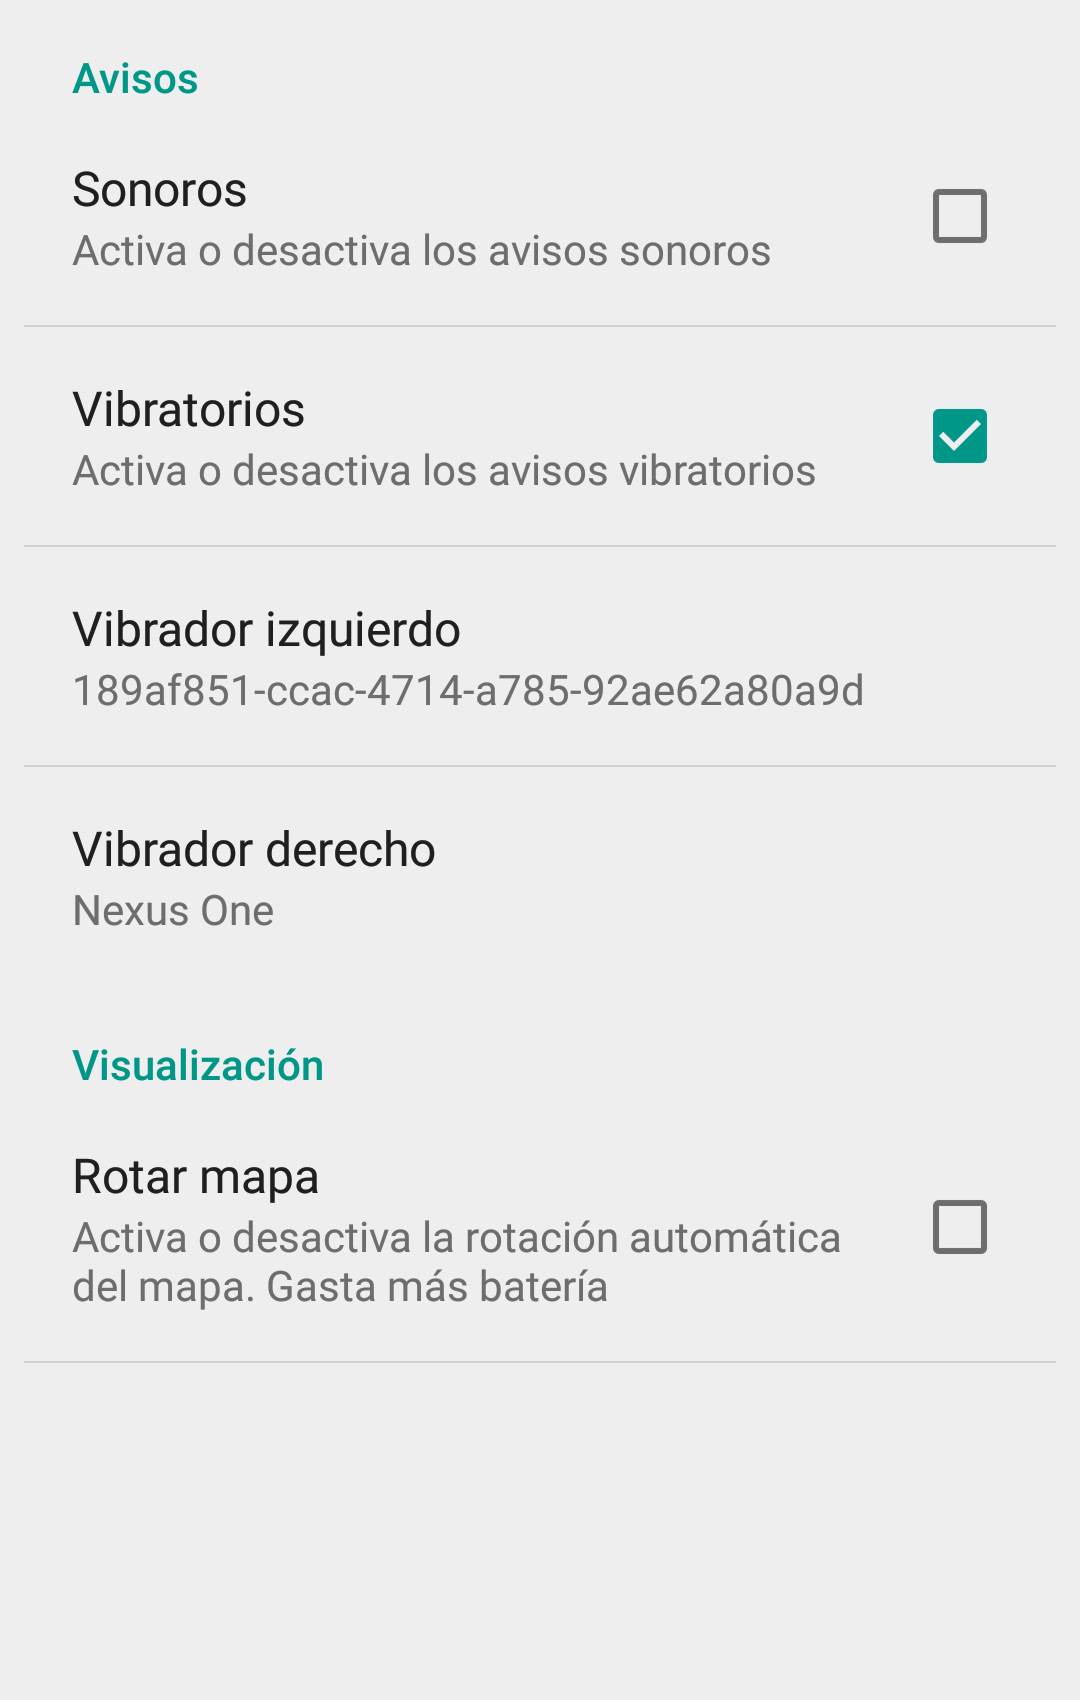
\includegraphics[width=0.85\textwidth]{/naviganto-opcionesconfiguradas.png}
      \caption{Opciones del caso de uso}
      \label{fig:navigantoOpcionesCasoDeUso}
    \end{center}
  \end{minipage}
\end{figure}

Este es el momento oportuno para ejecutar la aplicación \emph{NavigantoBluetooth} de nuestro otro
\emph{smartphone} y que se quede a la espera (ver
figura~\ref{fig:navigantoBluetoothIniciado}). También podríamos ejecutar la aplicación
\emph{NavigantoWear} en nuestro \emph{smartwatch} aunque no es necesario, esta aplicación puede
iniciarse sola.

\begin{figure}[!h]
  \begin{center}
    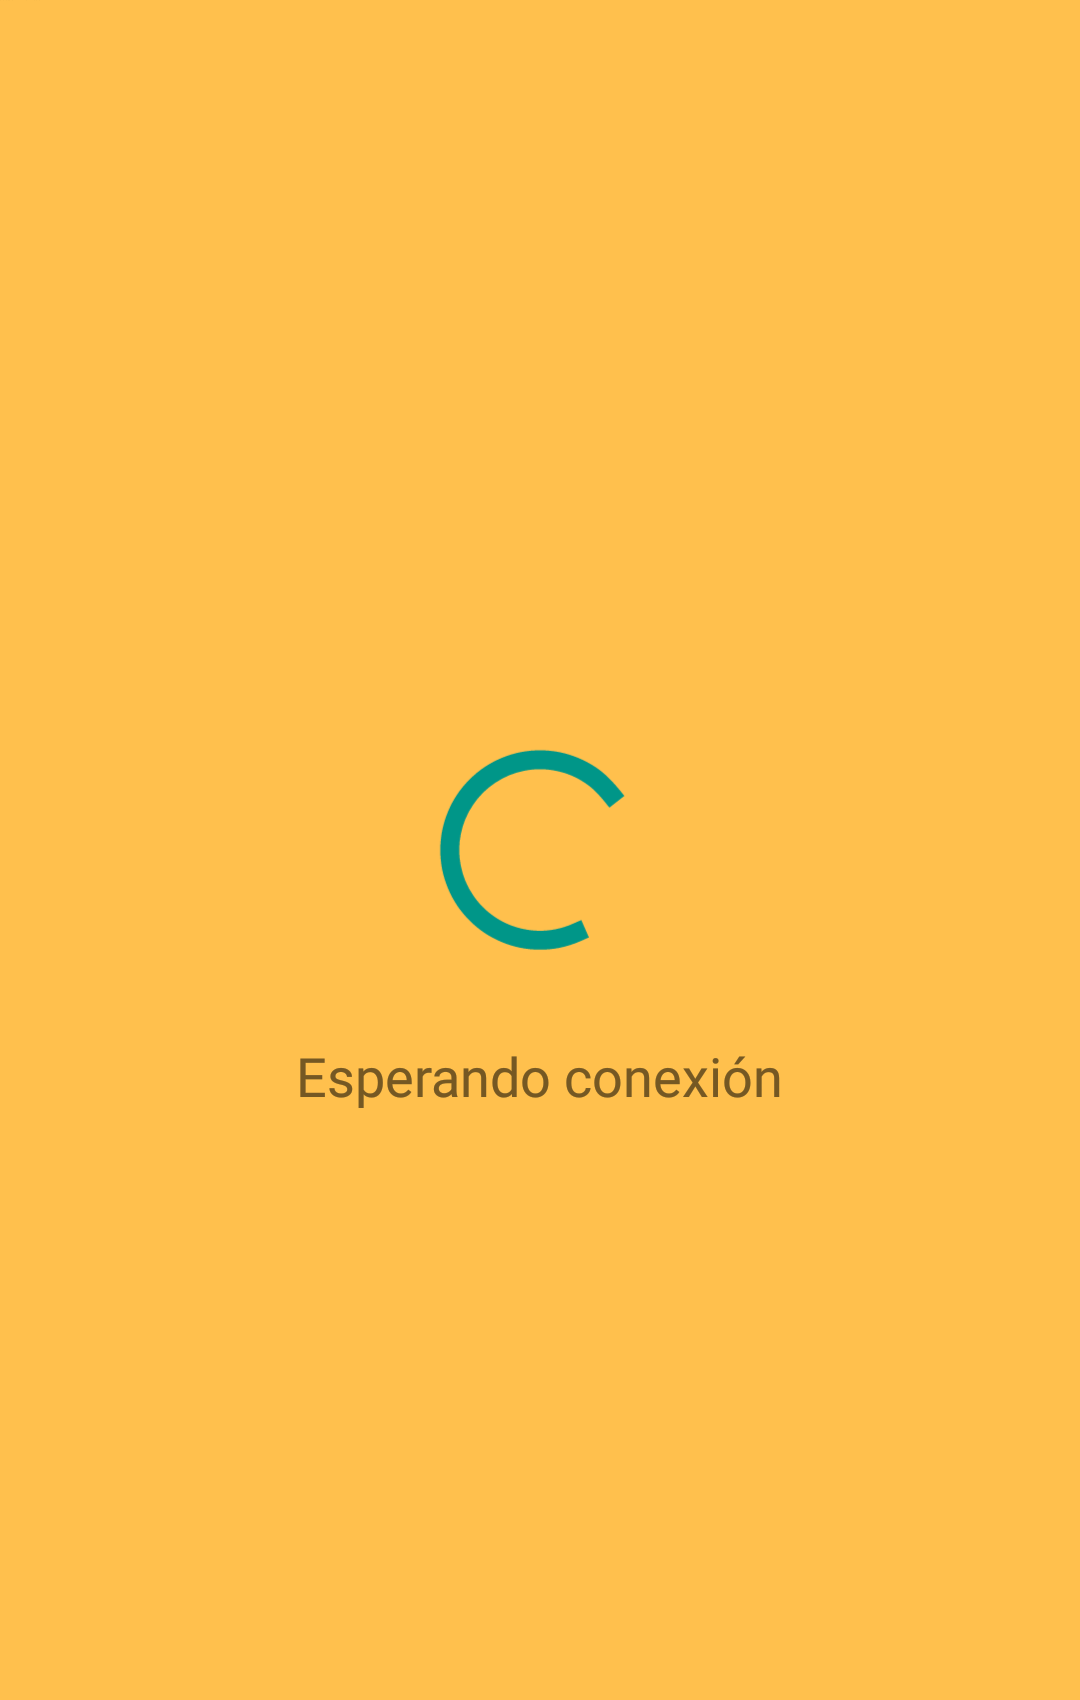
\includegraphics[width=0.425\textwidth]{/navigantobluetooth-ini.png}
    \caption{NavigantoBluetooth tras iniciarse, es decir, esperando conexión}
    \label{fig:navigantoBluetoothIniciado}
  \end{center}
\end{figure}

Ahora es el momento de pulsar la tecla de retroceso dentro de la opciones de \emph{Naviganto} para
que instantes después figuren los dos dispositivos como conectados (ver
figuras~\ref{fig:NavigantoBluetoothEsperando} y~\ref{fig:NavigantowearEsperando}).

\begin{figure}[!h]
  \begin{minipage}[b]{0.5\linewidth}
    \begin{center}
      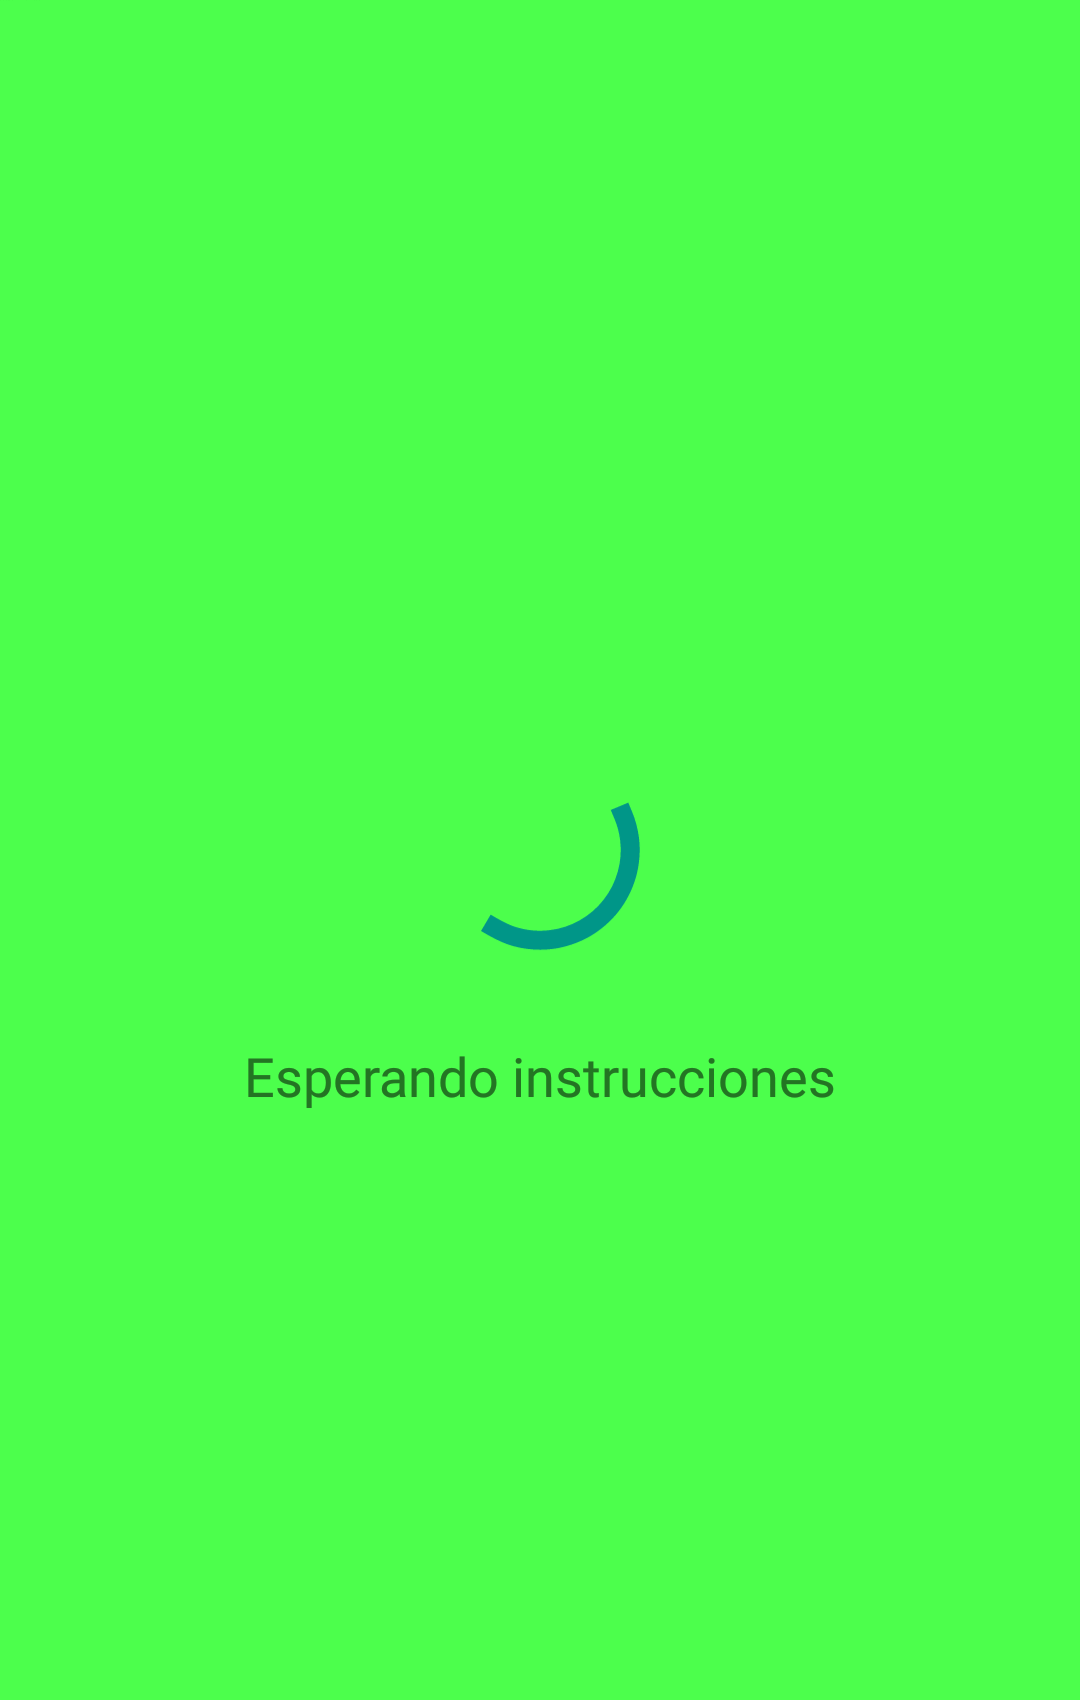
\includegraphics[width=0.85\textwidth]{/navigantobluetooth-esperando.png}
      \caption{NavigantoBluetooth esperando instrucciones}
      \label{fig:NavigantoBluetoothEsperando}
    \end{center}
  \end{minipage}
  \begin{minipage}[b]{0.5\linewidth}
    \begin{center}
      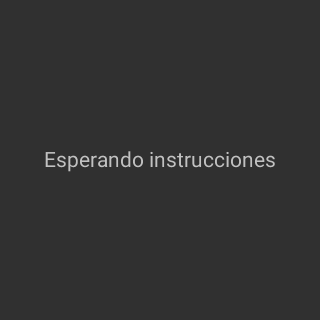
\includegraphics[width=0.85\textwidth]{/navigantowear-esperando.png}
      \caption{NavigantoWear esperando instrucciones}
      \label{fig:NavigantowearEsperando}
    \end{center}
  \end{minipage}
\end{figure}

Para comprobar que la configuración ha tenido éxito podemos seleccionar la opción de la barra
lateral de \emph{Naviganto} llamada \emph{Probar vibración} (ver
Figura~\ref{fig:navigantoBarra}). De esta forma, se mandará a \emph{NavigantoWear}, que está
configurado en la posición izquierda, la orden de vibrar durante 0.9 segundos. Acto seguido se le
mandará a \emph{NavigantoBluetooth}, que está configurado en la posición derecha, la orden de vibrar
durante otros 0.9 segundos. Gracias a esta comprobación estaremos seguros de que la configuración de
la vibración ha sido un éxito.

\subsection{La ruta}

Para introducir el destino al que deseamos ir, seleccionaremos la opción de la barra lateral
\emph{Seleccionar destino} tras lo cual nos aparecerá la figura~\ref{fig:navigantoDestinoIni}. Tras
seleccionar en el menú superior la opción \emph{Peatón}, introducir la dirección y pulsar en el
botón \emph{Buscar} se nos mostrará la figura~\ref{fig:navigantoDestinoBuscado}. Finalmente, tras
pinchar sobre el único resultado iniciaremos la navegación (ver figura~\ref{fig:navigantoRutaIni}).

\begin{figure}[!h]
  \begin{minipage}[b]{0.5\linewidth}
    \begin{center}
      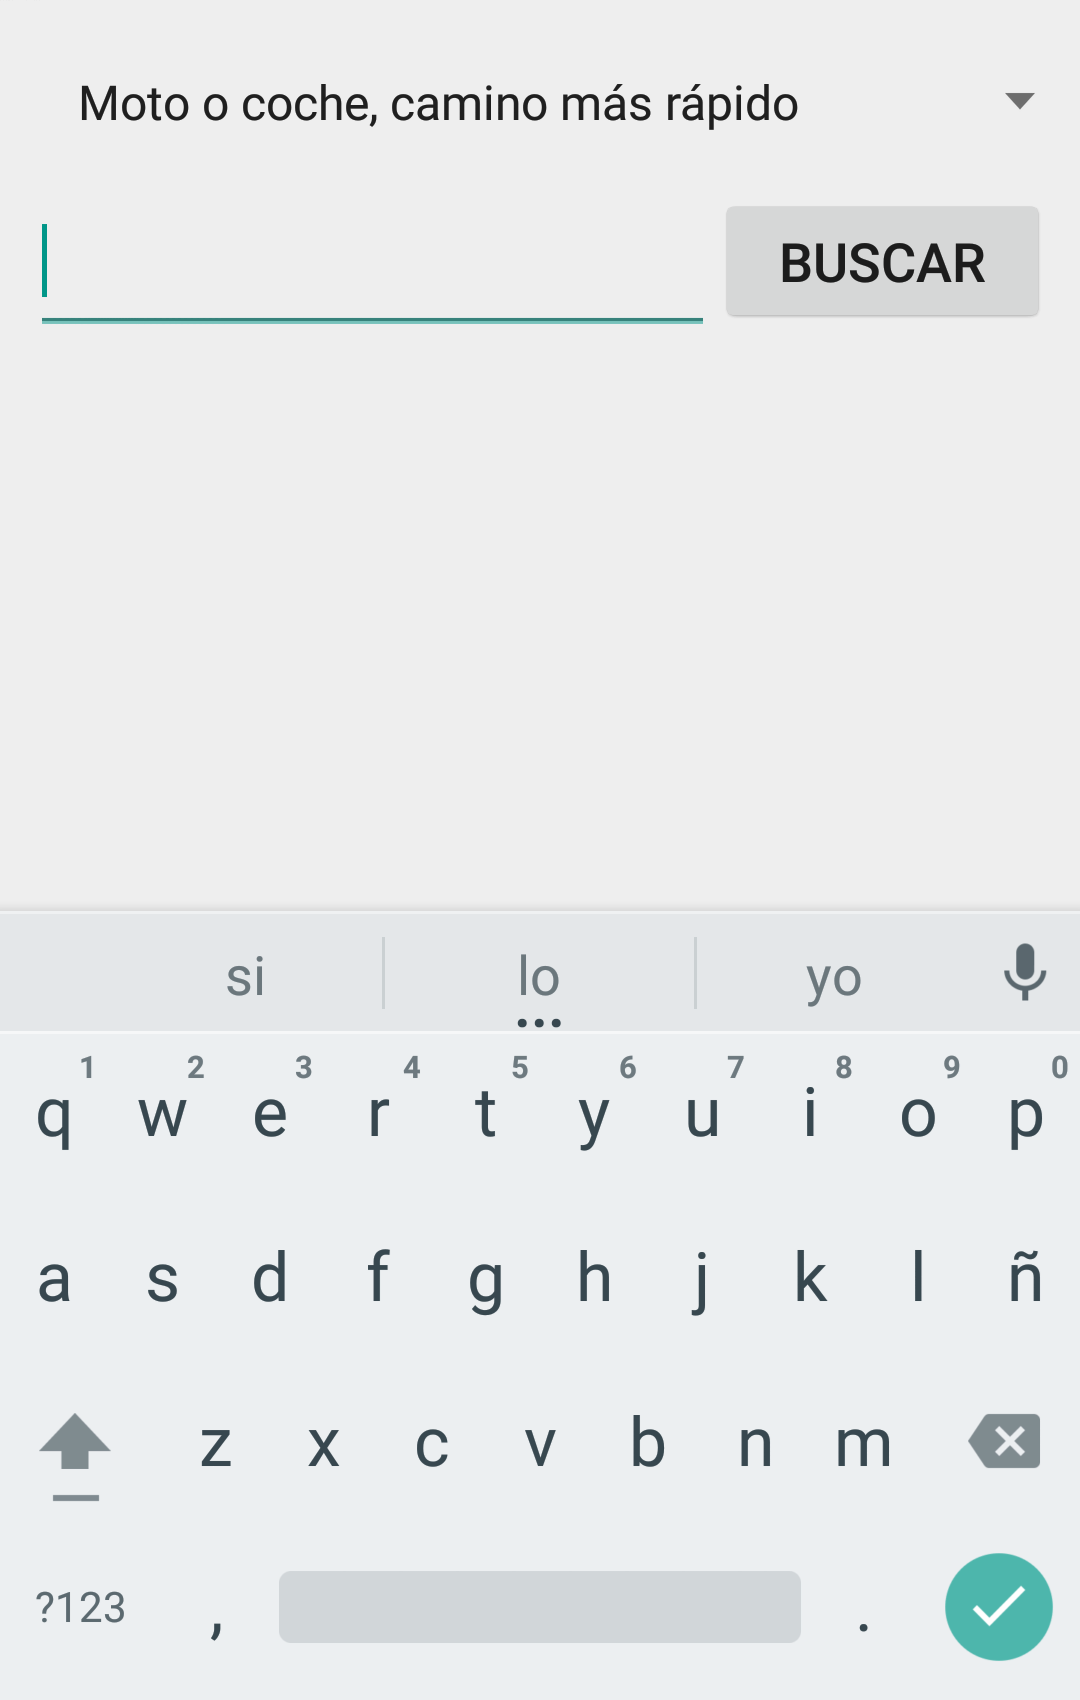
\includegraphics[width=0.85\textwidth]{/naviganto-destinoini.png}
      \caption{Buscador de destinos}
      \label{fig:navigantoDestinoIni}
    \end{center}
  \end{minipage}
  \begin{minipage}[b]{0.5\linewidth}
    \begin{center}
      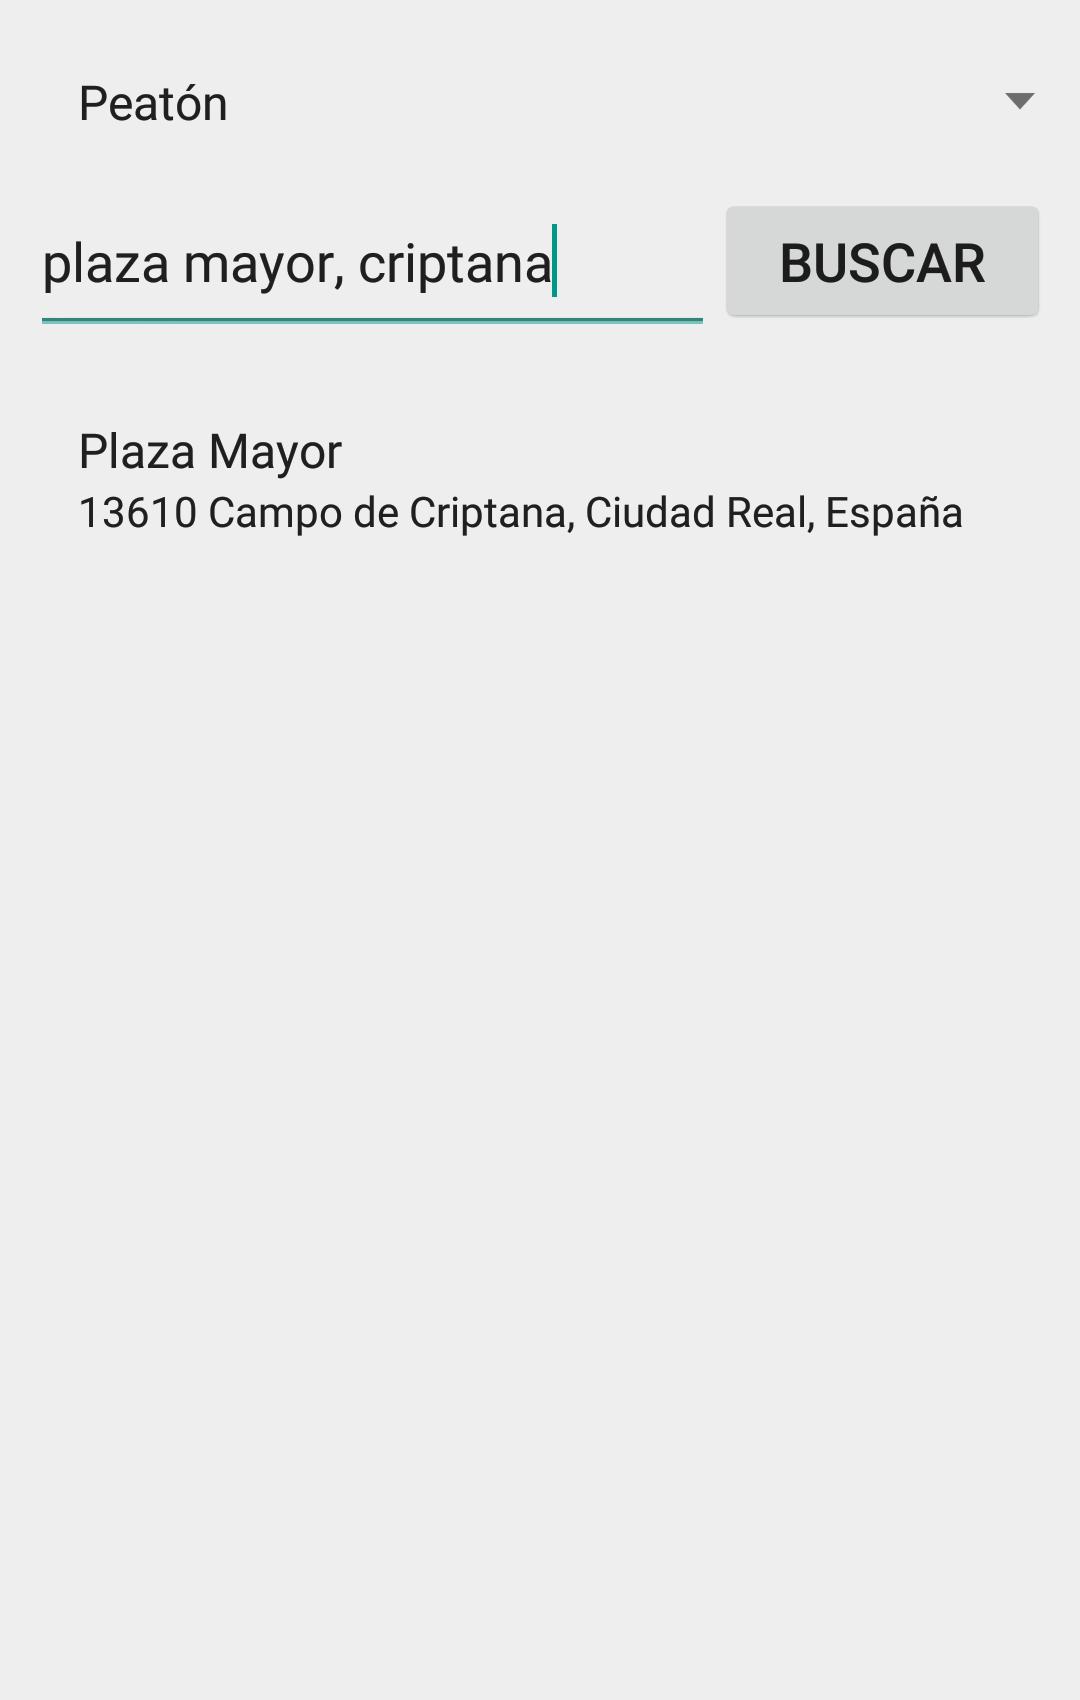
\includegraphics[width=0.85\textwidth]{/naviganto-destinobuscado.png}
      \caption{Búsqueda de destino}
      \label{fig:navigantoDestinoBuscado}
    \end{center}
  \end{minipage}
\end{figure}

Cuando iniciemos la marcha y lleguemos al primer giro (ver figura~\ref{fig:navigantoRutaPrimerGiro})
vibrará el \emph{smartphone} del bolsillo derecho del pantalón con la frecuencia determinada para
los giros (ver figura~\ref{fig:graficaGiro}). Más tarde, cuando lleguemos al segundo giro (ver
figura~\ref{fig:navigantoRutaSegundoGiro}) vibrará el \emph{smartwatch} con la misma
frecuencia. Finalmente, cuando lleguemos al destino (ver figura~\ref{fig:navigantoRutaFin}) vibrarán
ambos dispositivos con la frecuencia de \emph{destino alcanzado} (ver
figura~\ref{fig:graficaDestino}).

\begin{figure}[!h]
  \begin{minipage}[b]{0.5\linewidth}
    \begin{center}
      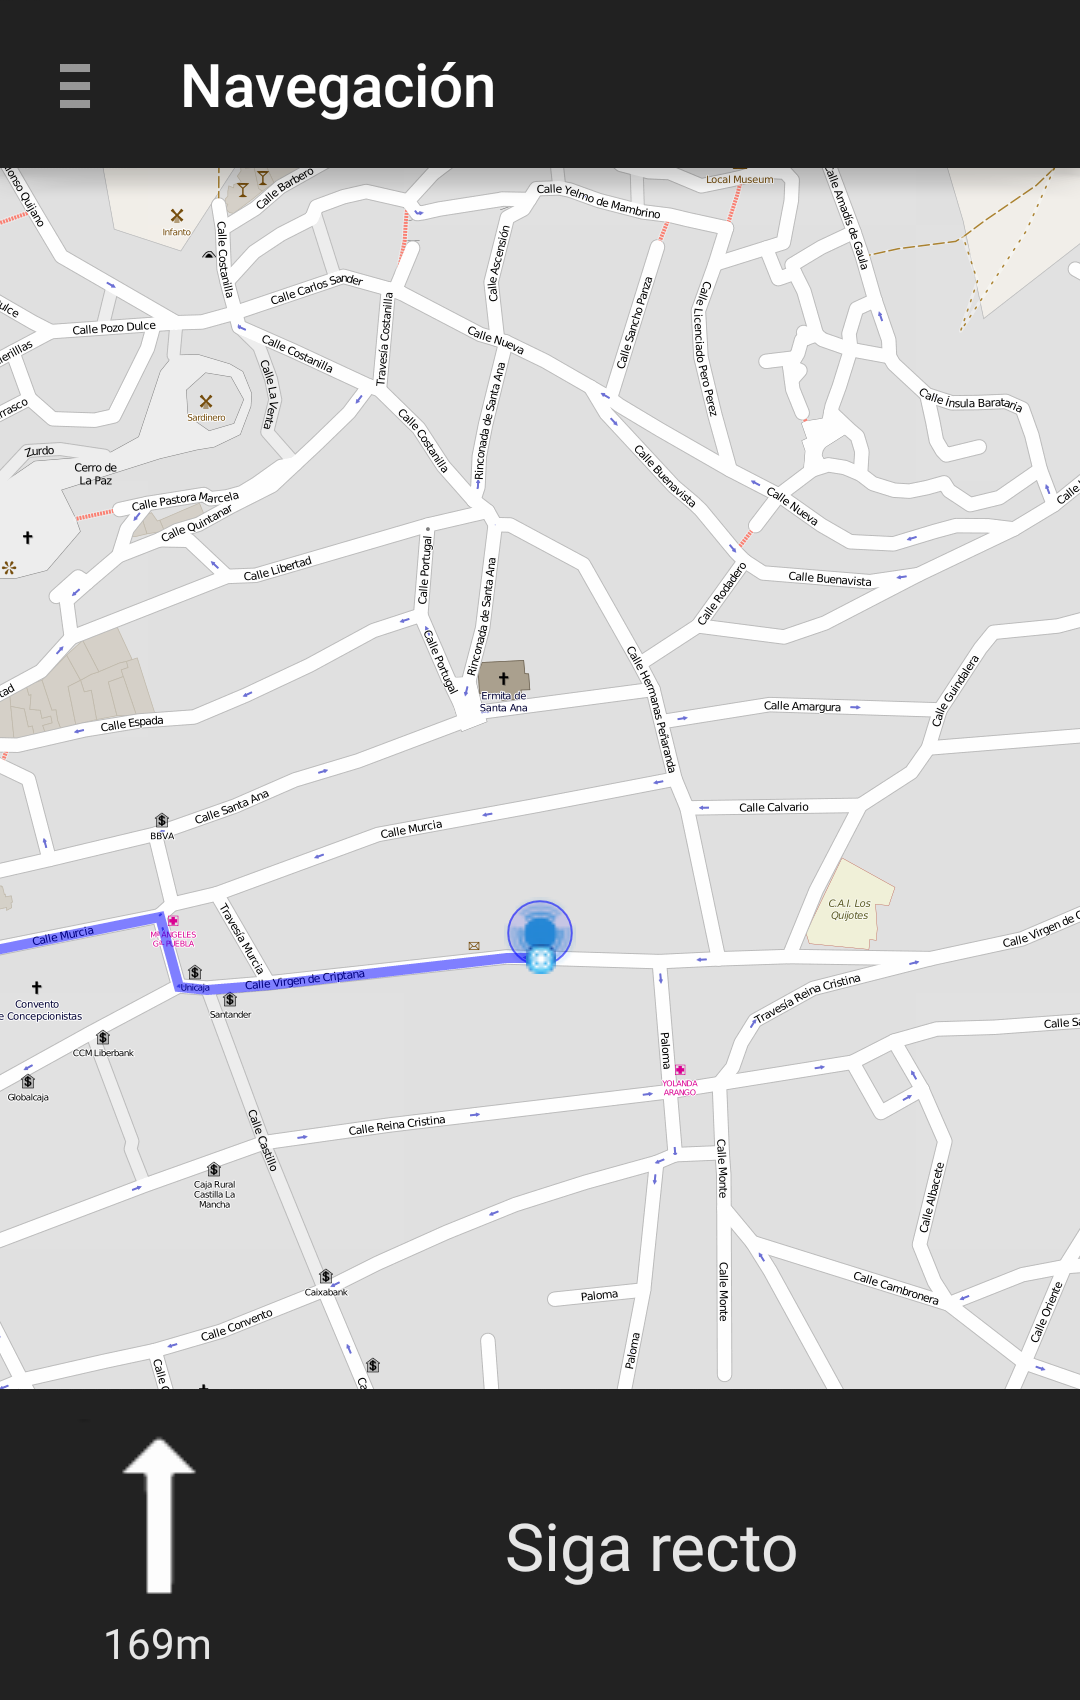
\includegraphics[width=0.85\textwidth]{/naviganto-rutaini.png}
      \caption{Inicio de ruta}
      \label{fig:navigantoRutaIni}
    \end{center}
  \end{minipage}
  \begin{minipage}[b]{0.5\linewidth}
    \begin{center}
      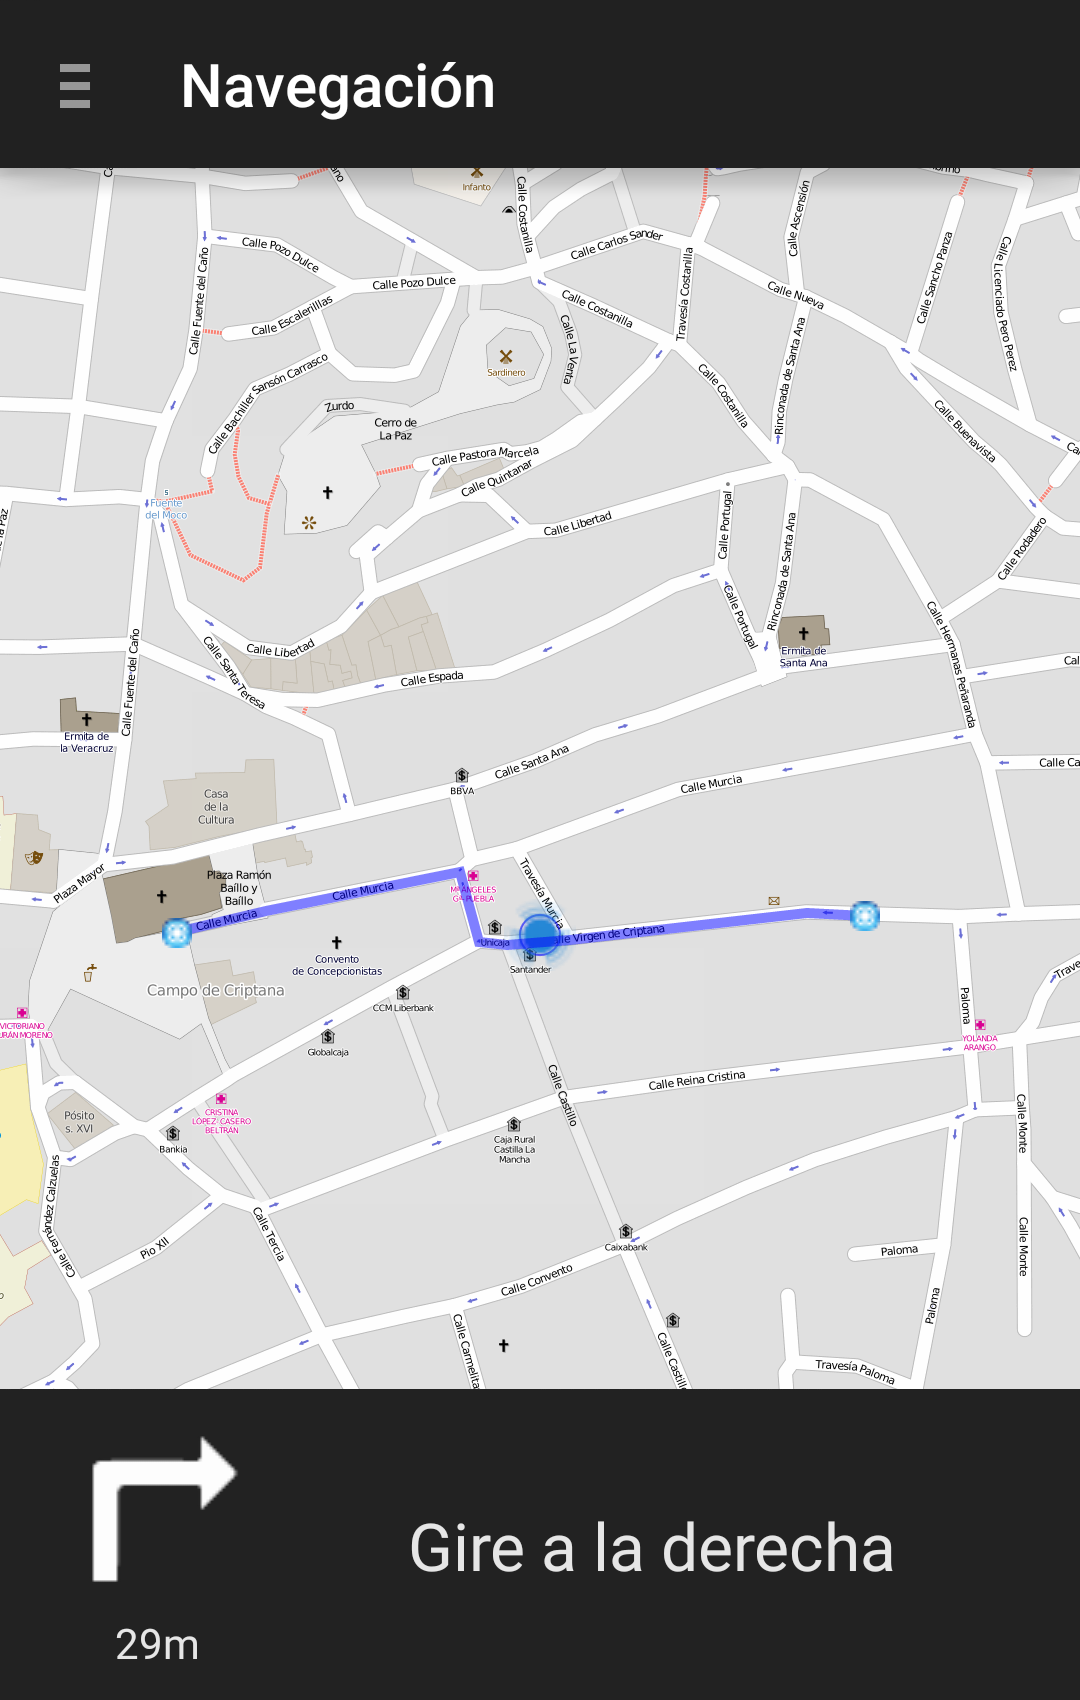
\includegraphics[width=0.85\textwidth]{/naviganto-rutaderecha.png}
      \caption{Primer giro de la ruta}
      \label{fig:navigantoRutaPrimerGiro}
    \end{center}
  \end{minipage}
\end{figure}

\begin{figure}[!h]
  \begin{minipage}[b]{0.5\linewidth}
    \begin{center}
      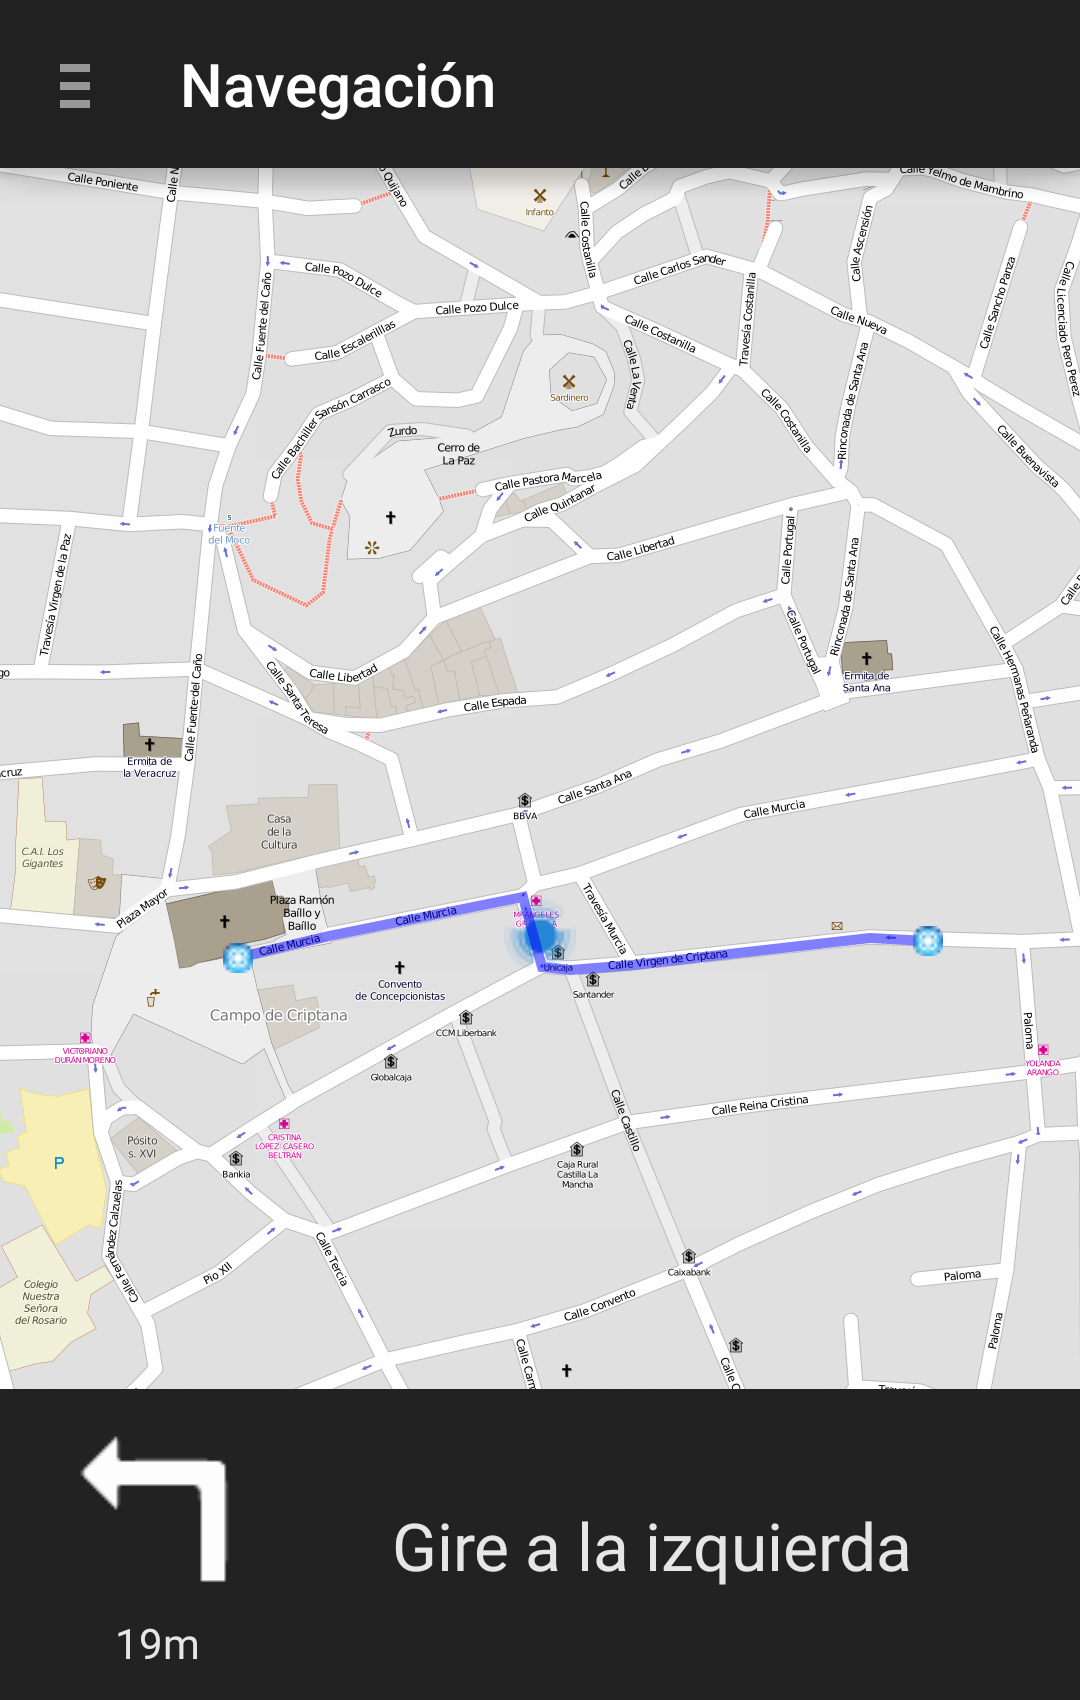
\includegraphics[width=0.85\textwidth]{/naviganto-rutaizquierda.png}
      \caption{Segundo giro de la ruta}
      \label{fig:navigantoRutaSegundoGiro}
    \end{center}
  \end{minipage}
  \begin{minipage}[b]{0.5\linewidth}
    \begin{center}
      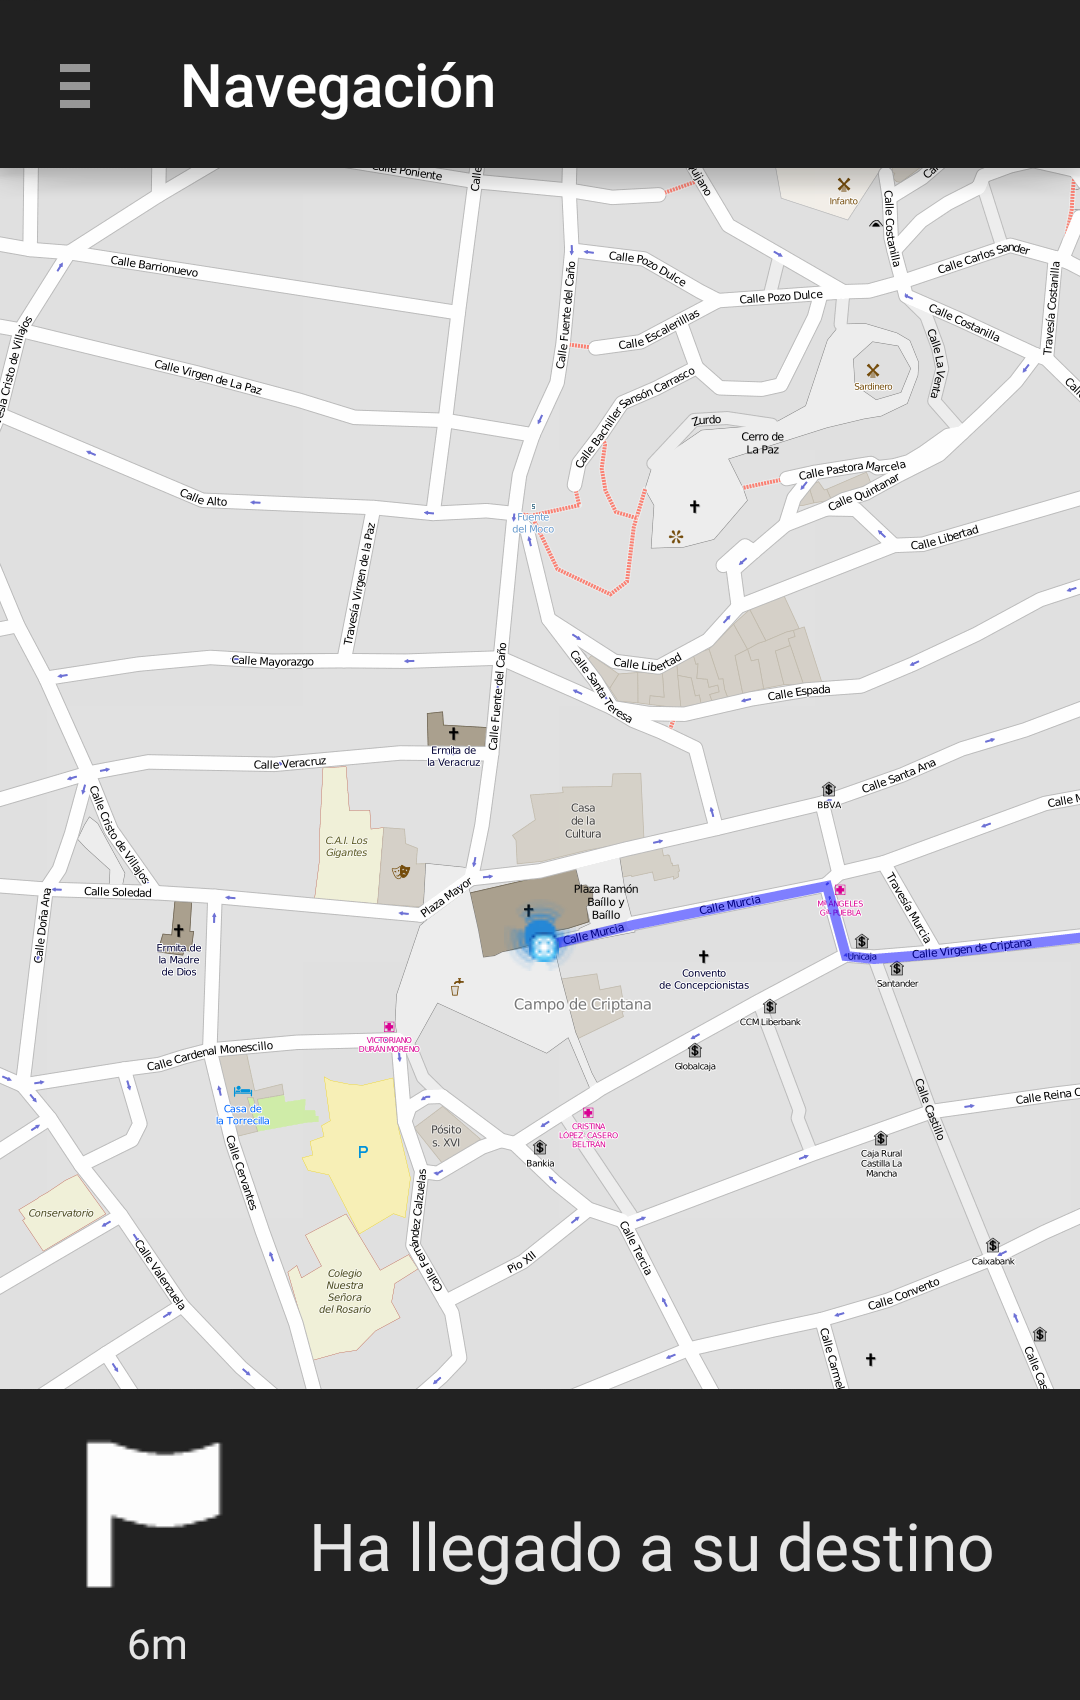
\includegraphics[width=0.85\textwidth]{/naviganto-rutafin.png}
      \caption{Llegada al destino, fin de la ruta}
      \label{fig:navigantoRutaFin}
    \end{center}
  \end{minipage}
\end{figure}

\newpage %<-- Sin el salto de página queda muy lioso...
\section{Repositorio}

El código desarrollado durante el transcurso del proyecto y la documentación de esta memoria se
encuentran disponibles en uno de los repositorios de \emph{BitBucket}:

\begin{listing}
https://bitbucket.org/cr4mos/tfg-sgpcmii
\end{listing}

Para descargar todo el repositorio puede utilizar el siguiente comando:

\begin{listing}[
  float=ht,
  language = Bash]
git clone https://bitbucket.org/cr4mos/tfg-sgpcmii.git
\end{listing}

Si sólo desea descargar las aplicaciones finales, diríjase a:

\begin{listing}
https://bitbucket.org/cr4mos/tfg-sgpcmii/src/e64e936da95e832f950617ebd50aec729aa9ee8c/Source/apk/?at=master
\end{listing}

Aunque si dispone de \emph{Play Store} en su \emph{smartphone} Android podrá descargar e instalar
las aplicaciones más fácilmente accediendo a:

\begin{listing}
https://play.google.com/store/apps/details?id=es.uclm.esi.tfg.naviganto
https://play.google.com/store/apps/details?id=es.uclm.esi.tfg.navigantobluetooth
\end{listing}

% Local Variables:
% TeX-master: "main.tex"
%  coding: utf-8
%  mode: latex
%  mode: flyspell
%  ispell-local-dictionary: "castellano8"
% End:
